\graphicspath{{chapters/chapter4/img/}}

\chapter{Results and discussion}
\label{cha:results}

This chapter is meant to show and discuss the results obtained from the application of the methods introduced in \Cref{cha:methods}.

\section{Emotion detection over time - by language}
\label{sec:emotion-by-language-res}

\begin{figure}[H]
	\centering
    	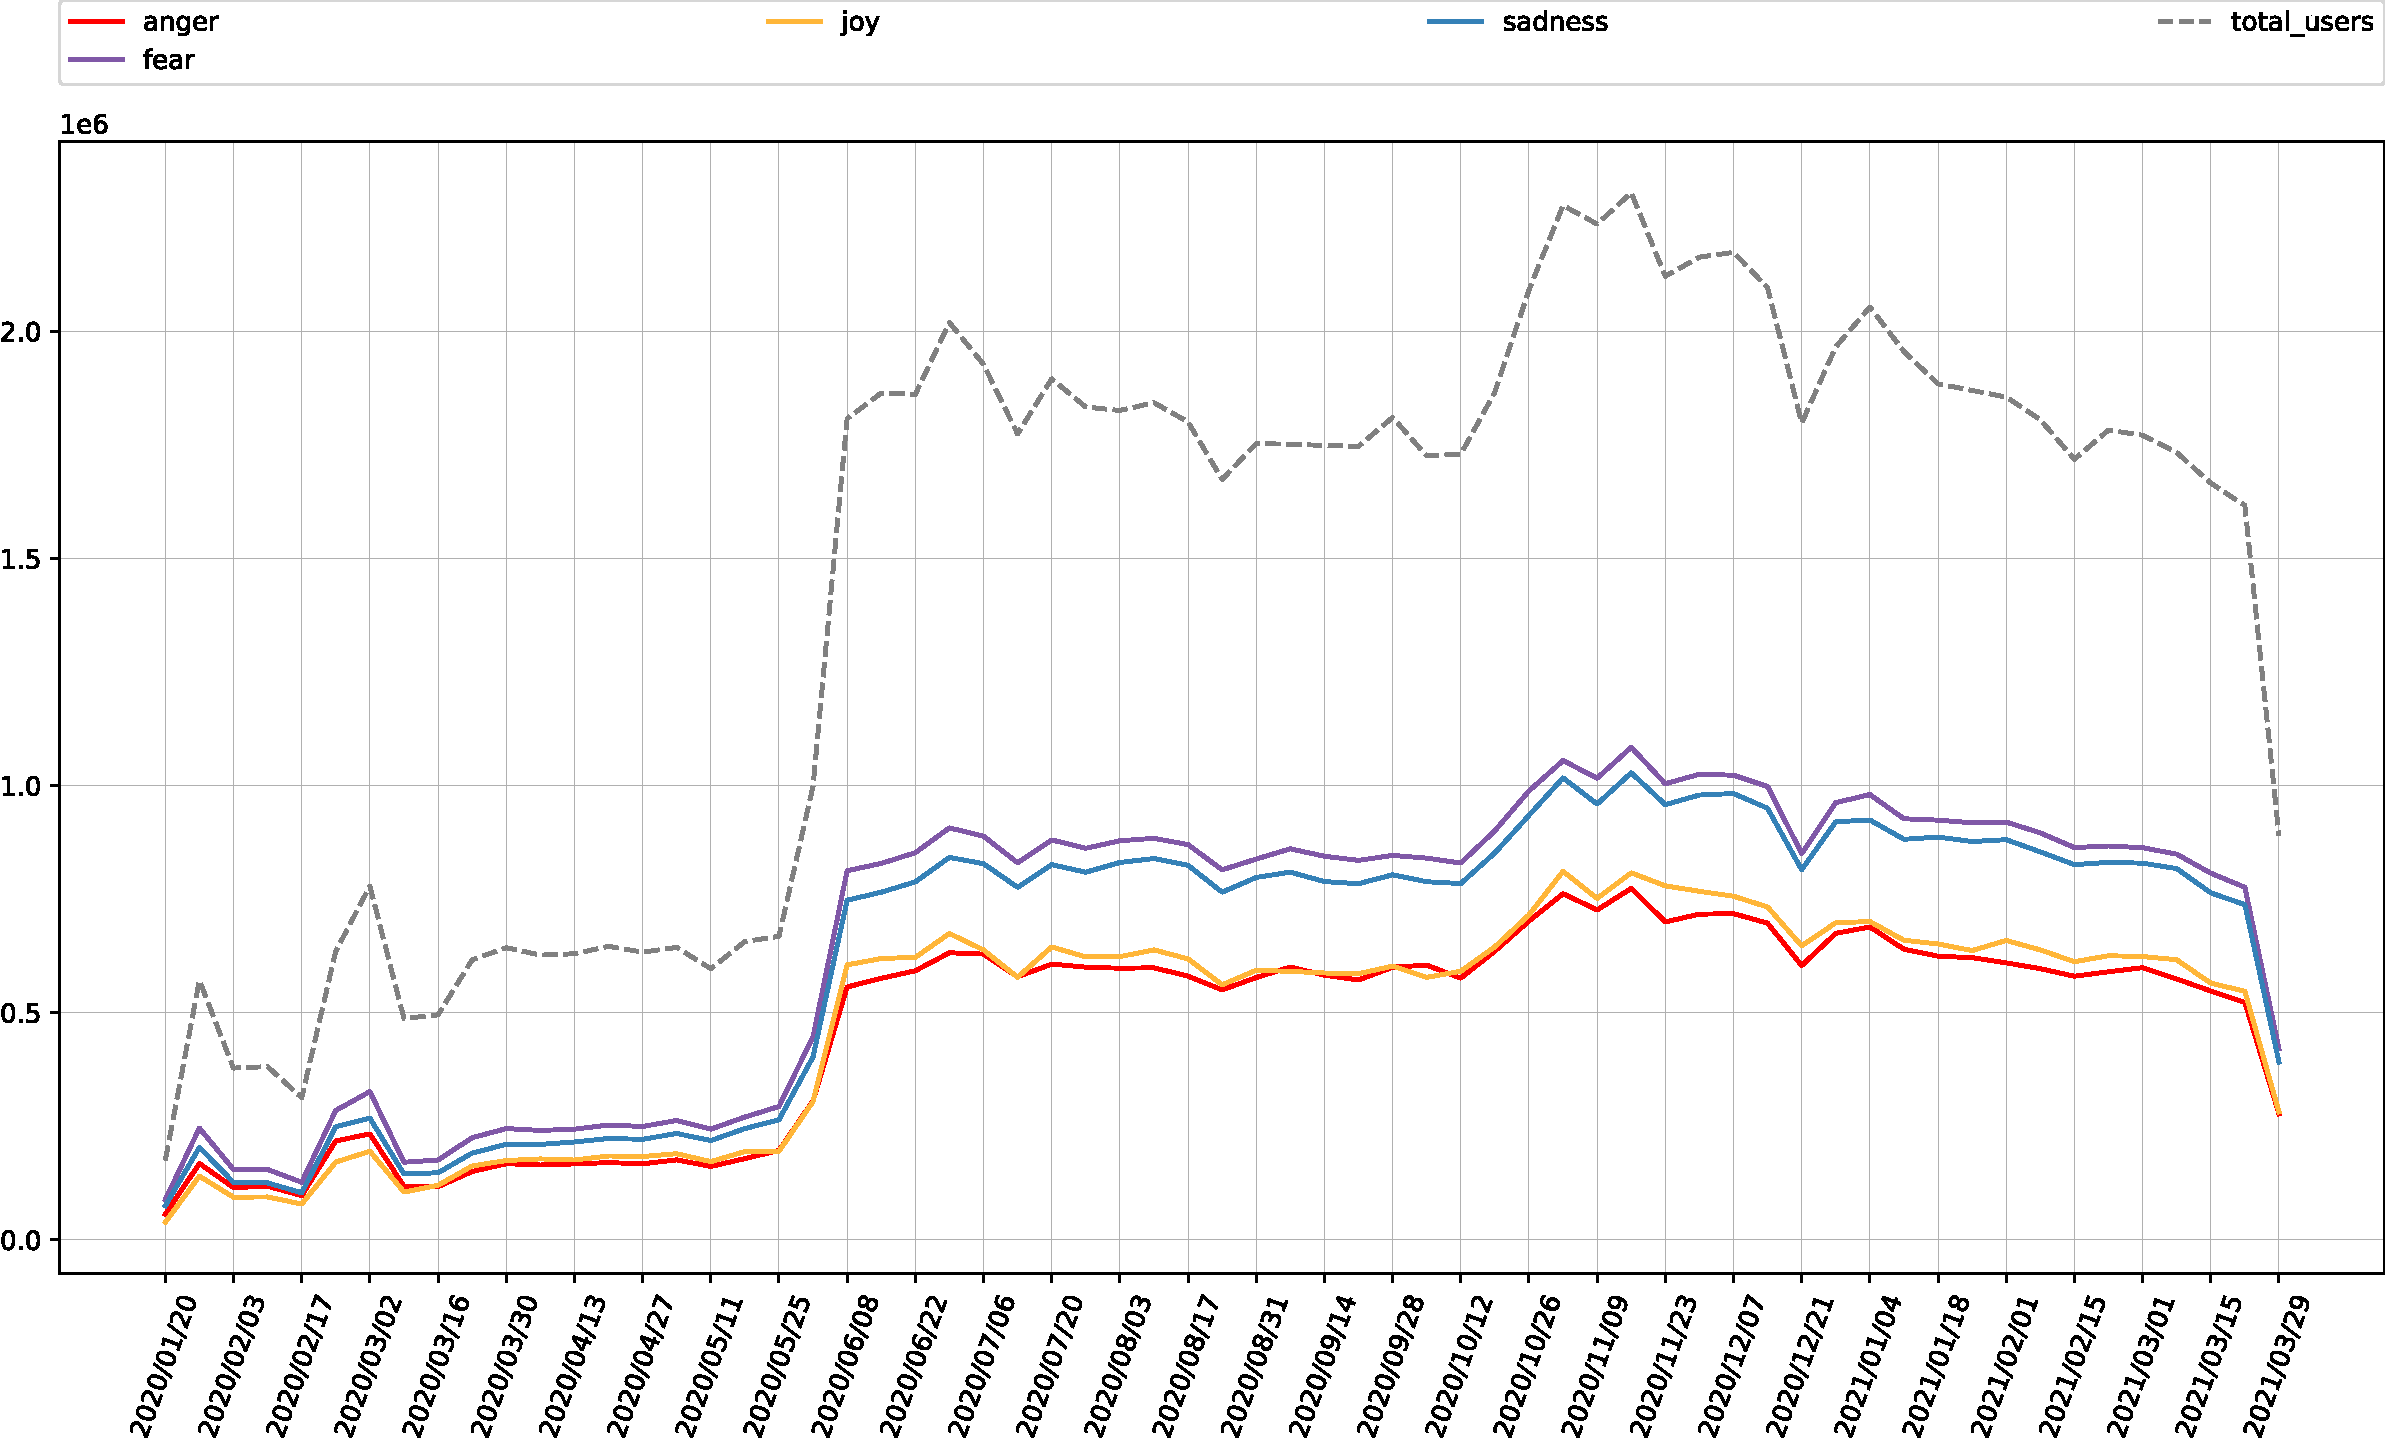
\includegraphics[scale=.35]{en_4_emotions_abs.svg}
    	\caption{Number of weekly users per emotion for the English tweets}
    	\label{fig:en-4-emotions-abs}
\end{figure}

\begin{figure}[H]
	\centering
    	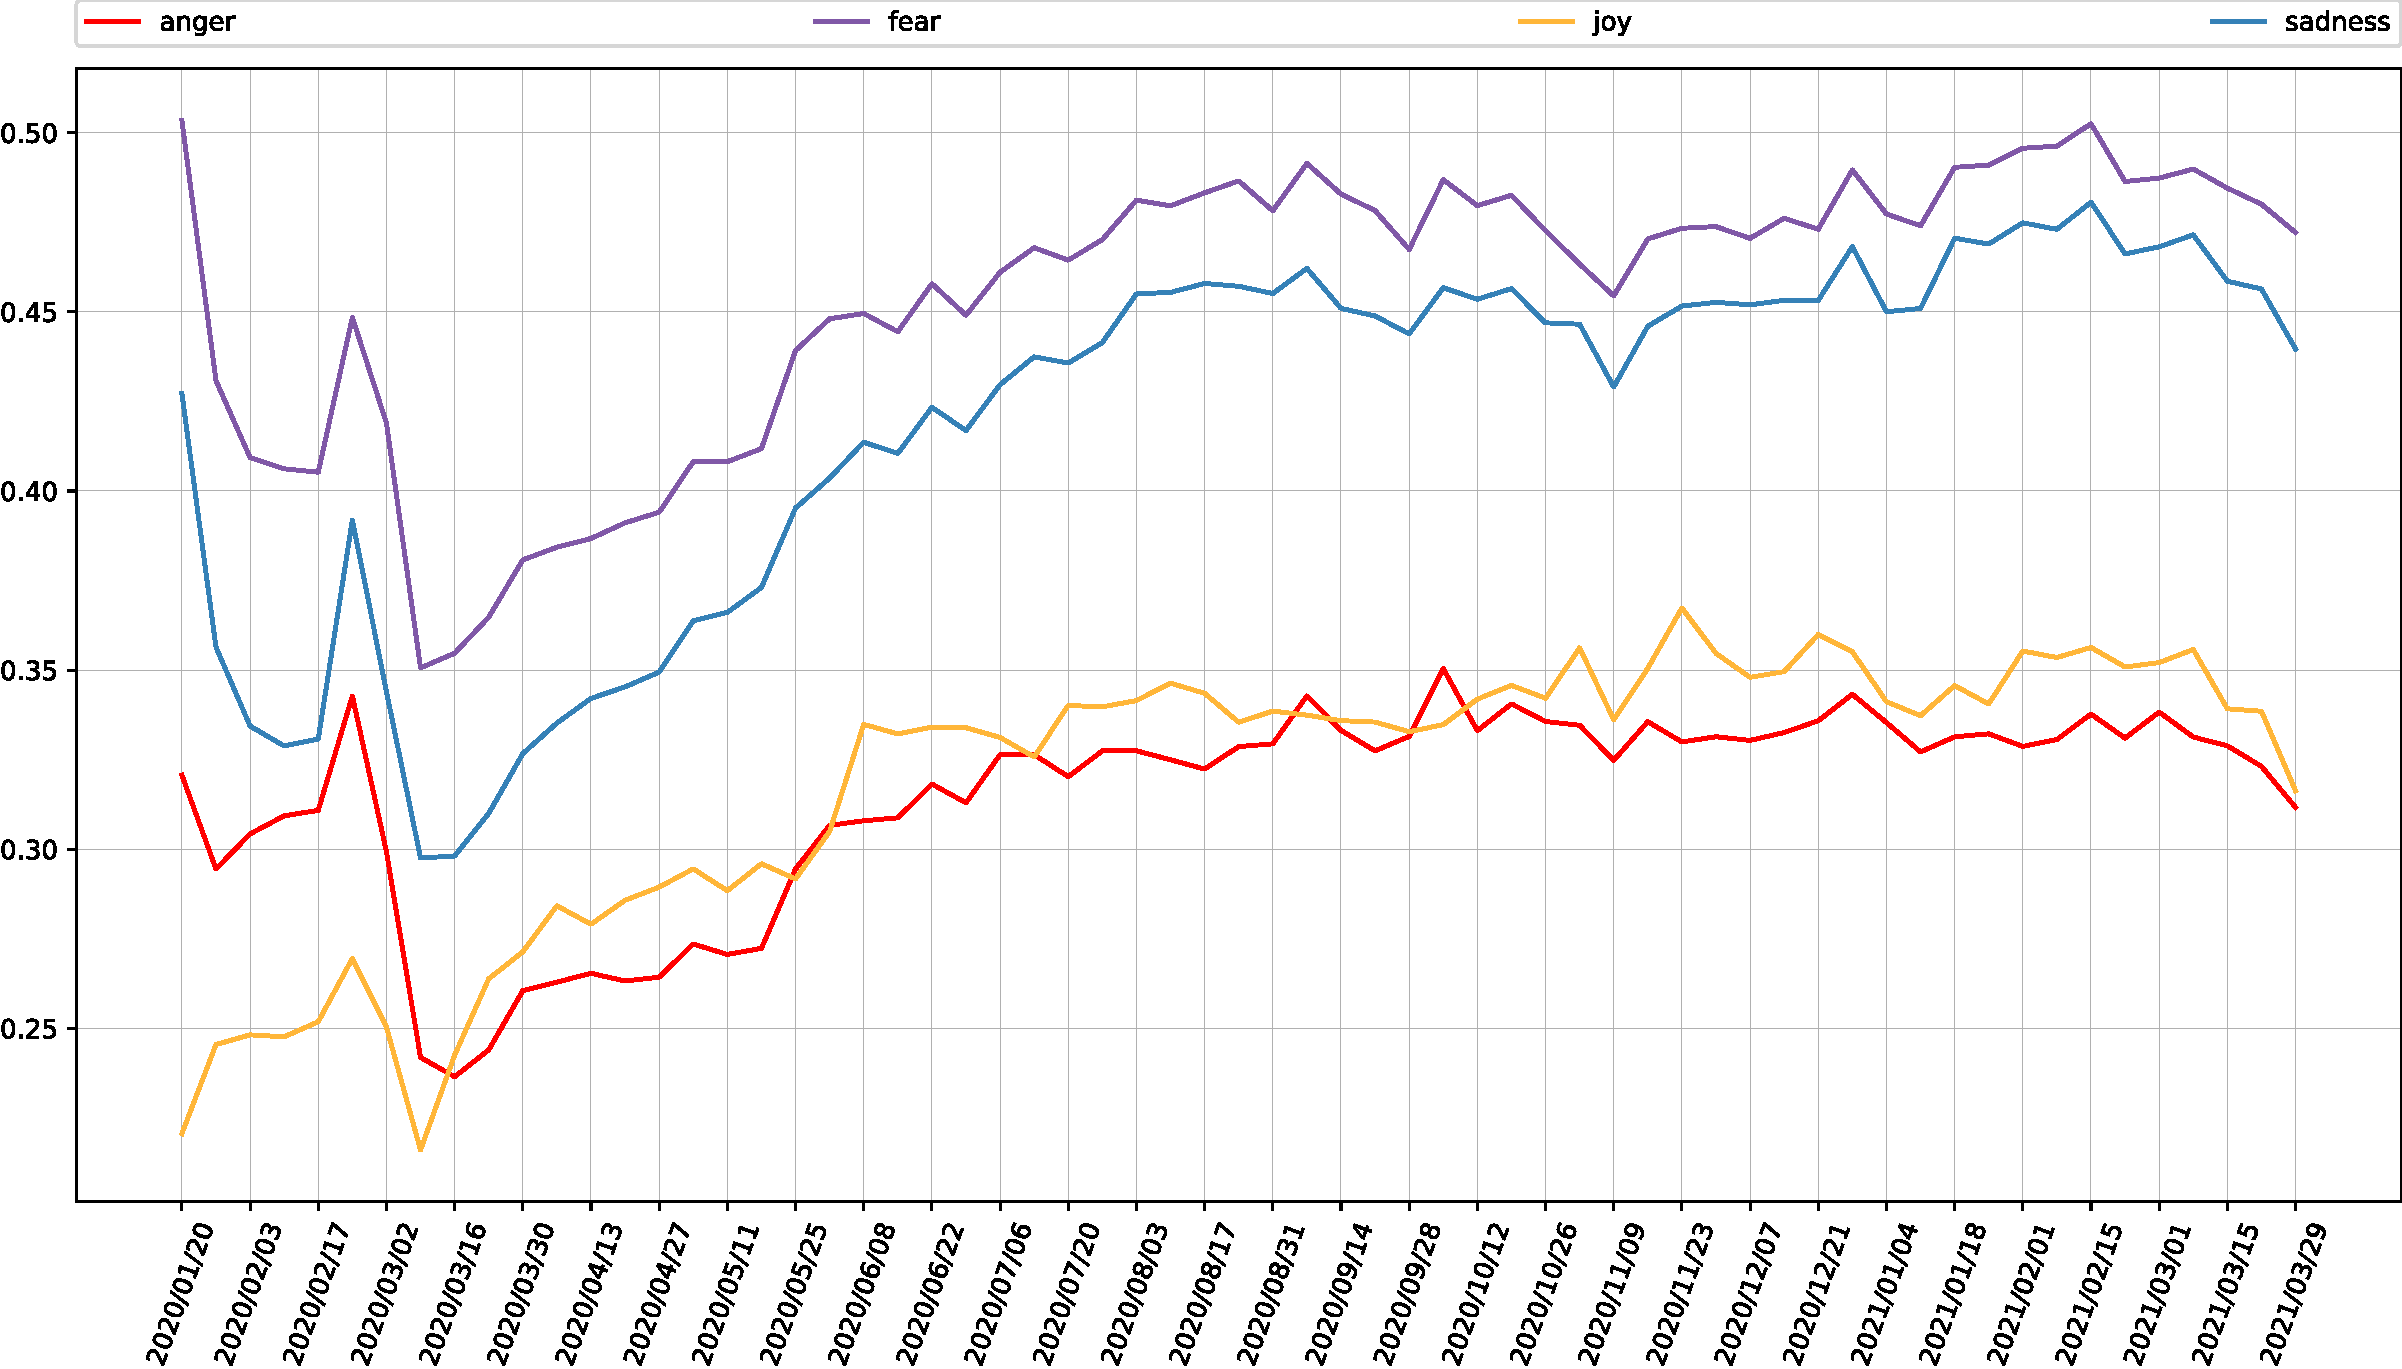
\includegraphics[scale=.35]{en_4_emotions.svg}
    	\caption{Proportion of weekly users per emotion for the English tweets}
    	\label{fig:en-4-emotions}
\end{figure}

\begin{figure}[H]
	\centering
    	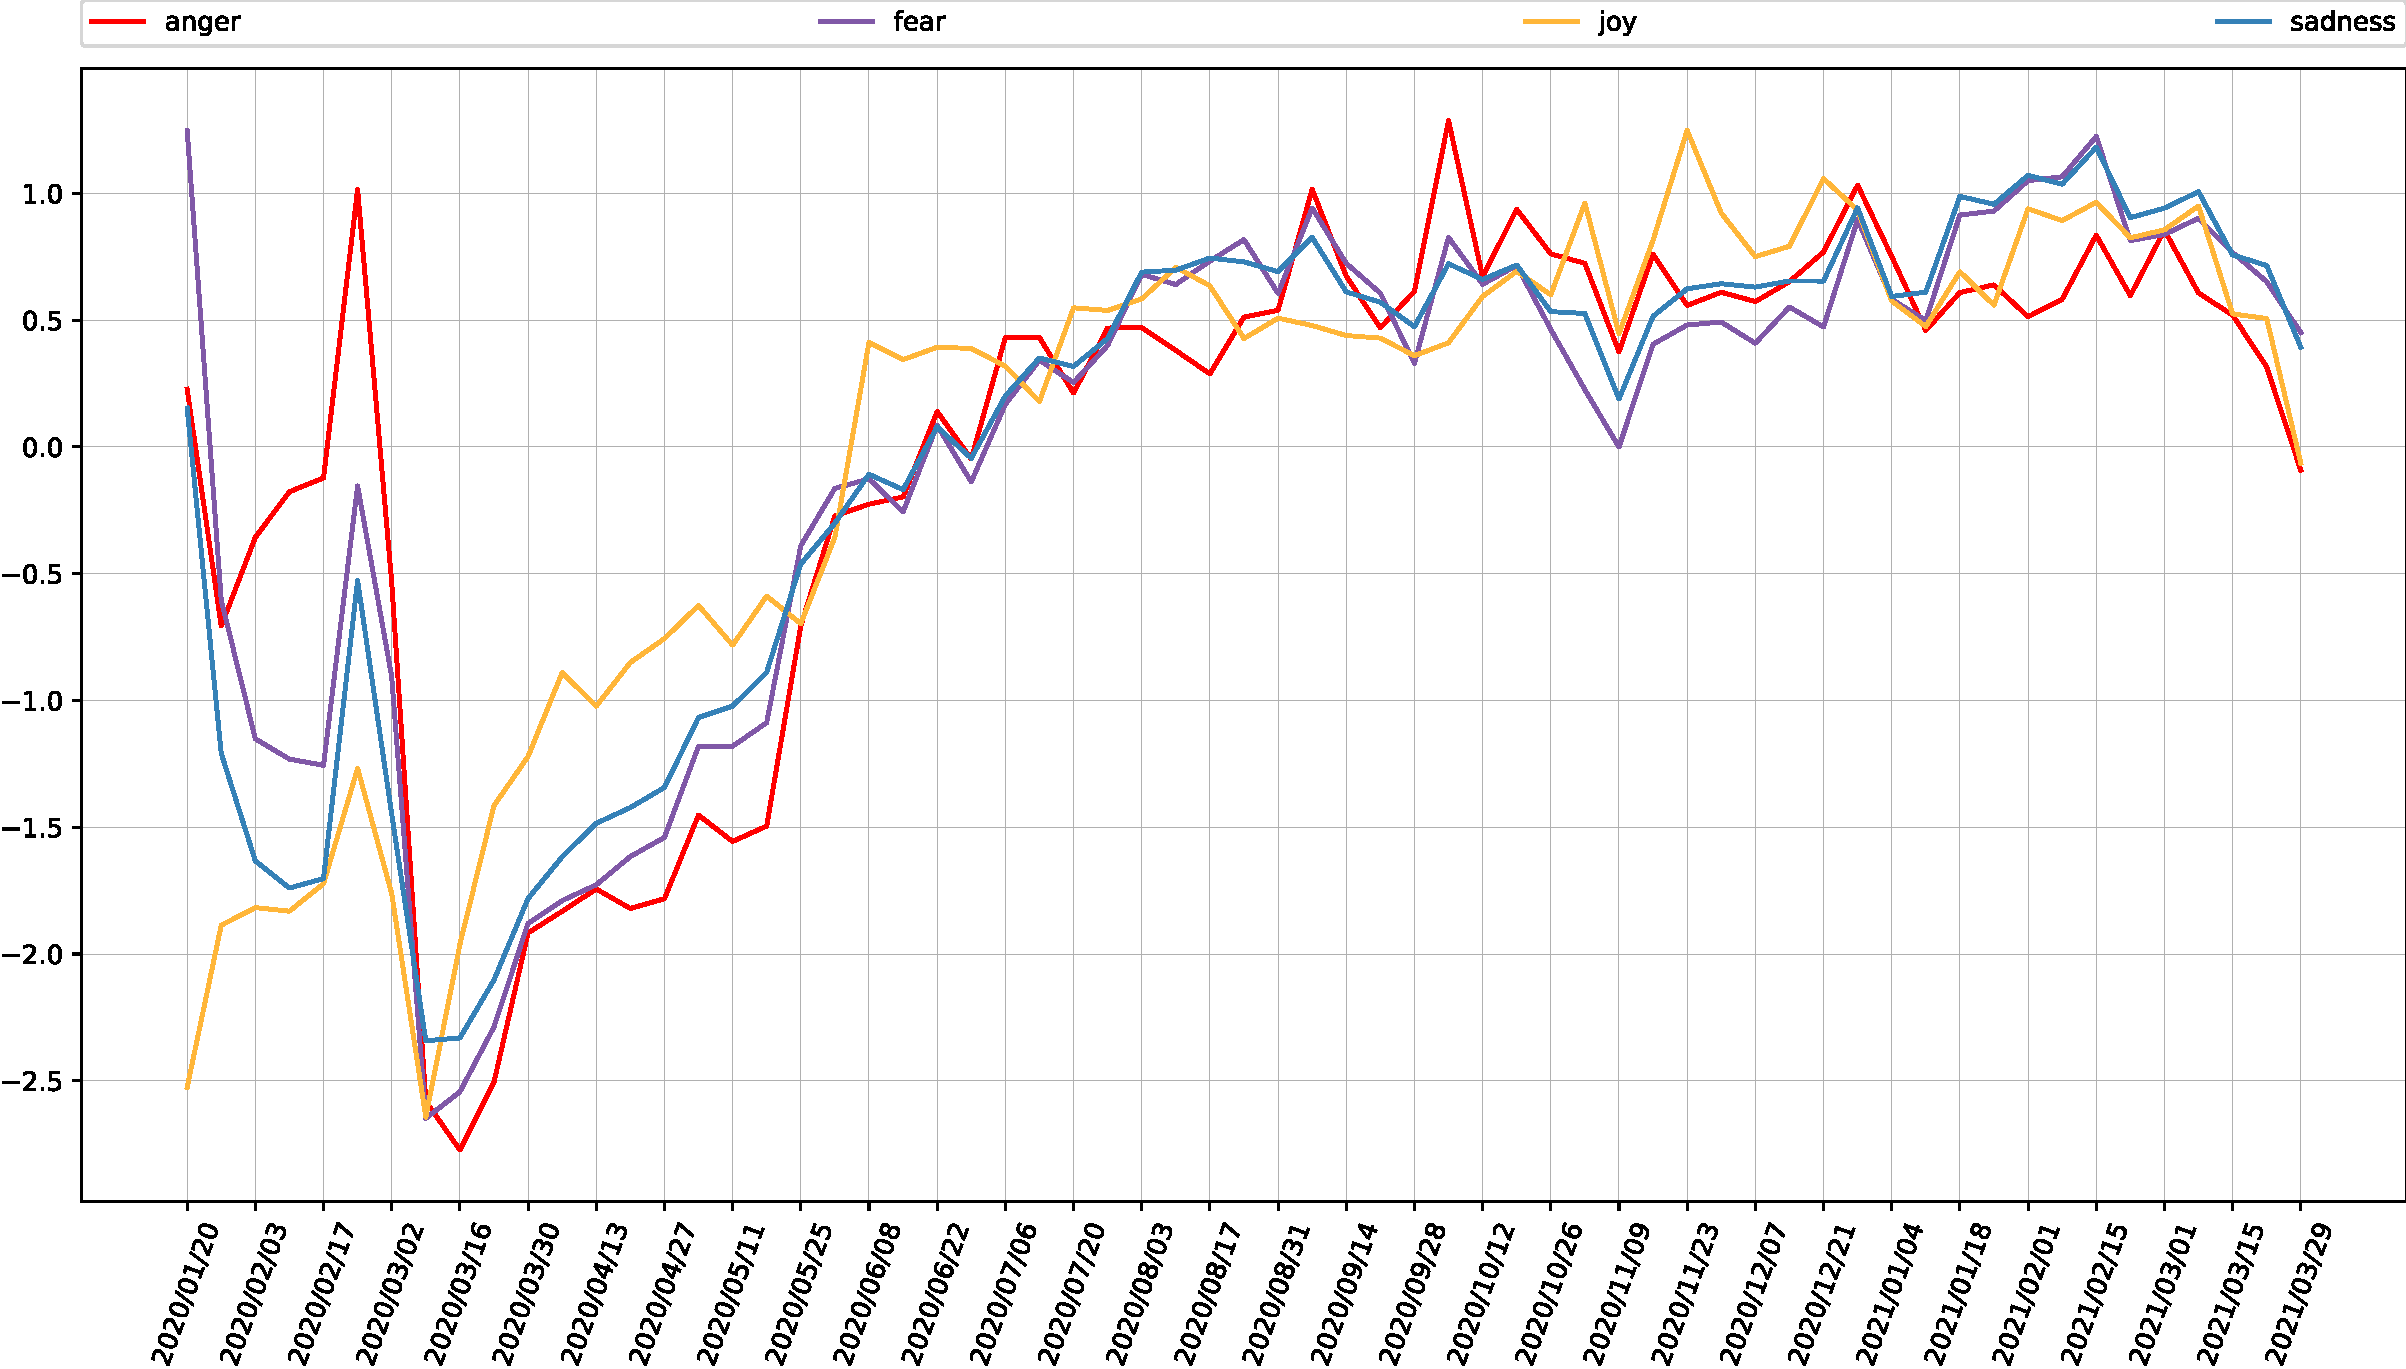
\includegraphics[scale=.35]{en_4_emotions_standardized.svg}
    	\caption{Z-score of weekly users per emotion for the English tweets}
    	\label{fig:en-4-emotions-std}
\end{figure}